\begin{homework}
  %% Conceptual Questions
  % Section 4.1 (Energy Equation)
  \question Thinking about the energy equation, how do we get the enthalpy term?  What concept gives us the additional term to change $u$ into $h$?
  
  \question What does the dot mean in $\dot{m}$, $\dot{W}$, and $\dot{Q}$?  What units do each of those terms have?
  
  % Section 4.2 (p-h Diagram)
  \question For an adiabatic process, how would we represent work on a $p$-$h$ diagram?
  
  \question Why are the constant temperature lines vertical to the left and right of the $p$-$h$ diagram?  Is enthalpy more dependent on temperature or pressure in those regions?
  
  \question Why is the constant temperature line horizontal in the central point of the diagram?  Assuming constant temperature, what is the primary property that would determine enthalpy in that region?
  
  % Section 4.3 (Components of Thermo Systems)
  \question Which components add or remove energy as work from a system?
  
  \question Which components add or remove energy as heat from a system?
  
  \question Which components move heat within the system?
  
  \question Which components do not add or remove energy as either work or heat?

  \question What limitations are placed on pumps and turbines? (i.e. where in the $p$-$h$ diagram are they allowed to operate?)
  
  % Section 4.4 (Basic Rankine Cycle)
  \question What four components are present in the Rankine cycle?
  
  \question Why do we sometimes neglect the energy to run the pump?
  
  \question How do we define efficiency for a Rankine cycle?  What are we ``getting out'' of the cycle?  What are we ``putting in''?
  
  % Section 4.5 (Rankine with Mods)
  \question What value did the reheat process add?  Thinking about Example \ref{ex:ch4_supercrit}, what would have happened without re-heating?  What would the quality have been at the outlet of the LP turbine?  Is that acceptable for turbines?
  
  \question How did the efficiency equation change when we considered a reheat?
  
  \question What value did regeneration add in Example \ref{ex:ch4FeedwaterHeater}? Without regeneration, what happens to the heat added in the steam generator?  What happens to the total work output? What happens to the efficiency?
  
  % Section 4.6 (Refrigeration)
  \question What has motivated the change in refrigerants over the years?
  
  \question What makes R1234yf preferable to R134a?  What makes it worse?
  
  \question Why do we use a throttle instead of a turbine for a refrigeration cycle?
  
  \question A furnace directly burns fuel to heat homes.  How does this differ from a heat pump?  What about electric space heaters?  For each, what are we paying for to get the end product of heat inside our house?
  
  \question Do refrigerators move heat from cold to hot? If so, how?
  \newpage
  %---------------------------------------------------------------------------
  %% Work-out Questions
  \question A small community of about 500 households have discovered an underground geothermal brine source that can be used to boil water at 100°C and would like to use this to generate power. The following diagram shows the initial design of a low pressure geothermal plant in which the water is boiled by the geothermal source to 100°C and subsequently superheated to 200°C by a wood-fired superheater. Notice that the high pressure of the system is at 100kPa allowing a convenient de-aerator to be placed at the pump outlet.
  \begin{center}
    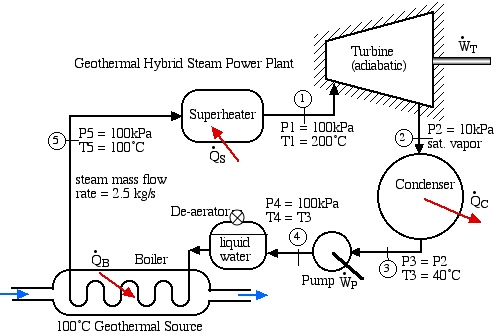
\includegraphics[width=0.75\textwidth]{ch4_HW_geo}
  \end{center}
  \begin{questionparts}
  \item Neatly sketch the complete cycle on the pressure-enthalpy $p$-$h$ diagram for water, indicating clearly all 5 stations on the diagram.
  \item Assuming that the turbine is adiabatic, determine the power output of the turbine \answer{[729kW]}.
  \item Assuming that the feedwater pump is adiabatic, and that the compressed liquid experiences no change in temperature while passing through the pump, determine the power required to drive the pump \answer{ [0.23kW]}.
  \item Using steam tables, determine the heat transferred to the boiler \answer{ [6271kW]} as well as the heat transferred to the superheater \answer{ [500kW]}.
  \item Determine the overall thermal efficiency $\eta_{th}$ of this power plant \answer{ [11\%]}. (Thermal efficiency is defined as the net work done by the system (turbine and feedwater pump) divided by the total heat supplied externally).  Is this the best measure of efficiency for this power plant?
  \item Discuss the proposed system with respect to its environmental impact and feasibility. Is this a well designed system? What do you consider to be the major advantages and disadvantages of this system? Your discussion should include a comparison of the external fuel used and the turbine power.
  \end{questionparts}
\newpage
  \question We wish to evaluate the proposed Solar-Pond Steam Power Plant shown in the following diagram. A solar pond is a large body of water having a varying salinity gradient (halocline) which traps the sun's energy such that the storage layer at the bottom of the pond can reach temperatures of greater than 100°C. The diagram following shows the initial design of a low pressure solar-pond steam power plant, using the storage layer as the boiler heat source, and the upper layer as the heat sink. Notice the wood-fired superheater in which the steam at the outlet of the boiler is heated from 100°C to 250°C.
  \begin{center}
     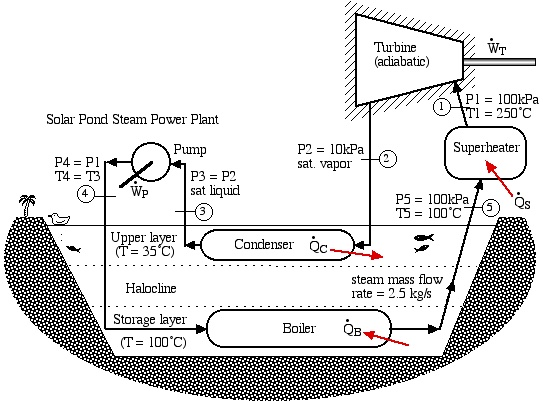
\includegraphics[width=0.75\textwidth]{ch4_HW_solar}
  \end{center}
  \begin{questionparts}
  \item Neatly sketch the complete cycle on the pressure-enthalpy $p$-$h$ diagram for water, indicating clearly all 5 stations on the diagram.
  \item Assuming that the turbine is adiabatic, determine the power output of the turbine \answer{ [976kW]}.
  \item Assuming that the feedwater pump is adiabatic, and that the compressed liquid experiences no change in temperature while passing through the pump, determine the power required to drive the pump \answer{ [0.23kW]}.
  \item Using steam tables, determine the heat transferred to the boiler \answer{ [6210kW]} as well as the heat transferred to the superheater \answer{ [747kW]}.
  \item Determine the overall thermal efficiency $\eta_{th}$ of this power plant \answer{ [14\%]}. (Thermal efficiency is defined as the net work done by the system (turbine and feedwater pump) divided by the total heat supplied externally).  Is this the best measure of efficiency for this power plant?
  \item Discuss the proposed system with respect to its environmental impact and feasibility. Is this a well designed system? What do you consider to be the major advantages and disadvantages of this system? Your discussion should include a comparison of the external fuel used and the turbine power.
  \end{questionparts}
  \question In an effort to decentralize the power grid and utilize the waste heat which accompanies power generation, the Athenai Power Consulting Corp. has proposed a Cogeneration system for O'Bleness Hospital to provide both 500 kW electric power and hot water at 60°C. The basic approach to this unique design is shown in the following schematic diagram:
  \begin{center}
    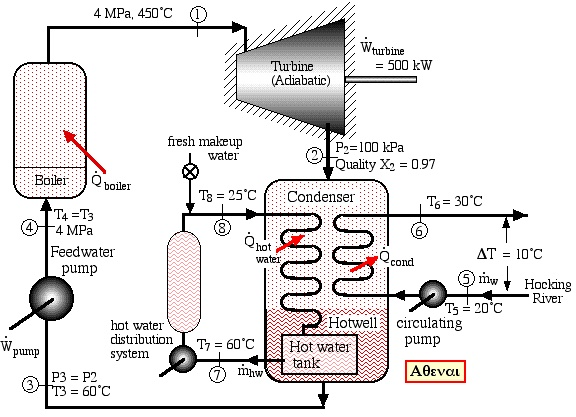
\includegraphics[width=0.75\textwidth]{ch4_HW_cogen}
  \end{center}
  \begin{questionparts}
  \item Neatly sketch the complete cycle on the pressure-enthalpy $p$-$h$ diagram for water, indicating clearly all 8 stations on the diagram.
  \item Determine the mass flow rate of the steam through the cycle required in order to provide the turbine output power of 500kW \answer{[0.691 kg/s]}.
  \item Determine the power required to drive the feedwater pump \answer{ [2.69 kW]}.
  \item Determine the overall thermal efficiency $\eta_{th}$ of this power plant. (Recall that thermal efficiency is defined as the net work done divided by the total heat supplied externally to the boiler \answer{[23\%]}.
  \item Determine the cooling power in the condenser required to condense the steam exiting the turbine at station (2) and subcool the condensed steam to 60°C at station (3) \answer{[1628 kW]}.
  \item Assuming that the water in the hot water distribution system is heated from 25°C to 60°C, and that no river cooling is provided, determine the mass flow rate of the hot water required to subcool the condenser water to 60°C \answer{ [11.1 kg/s]}
  \item In the lull period when no hot water is required, determine the mass flow rate of water from the Hocking River required to subcool the condenser water to 60°C. Note that the river water temperature rise must not exceed 10°C \answer{ [39 kg/s]}.
  \item Discuss the proposed system with respect to its environmental impact and feasibility.
  \end{questionparts}
  \question We wish to do a preliminary thermodynamic evaluation of a refrigeration system designed for home usage which will use refrigerant R134a. Consider the following system flow diagram:
  \begin{center}
    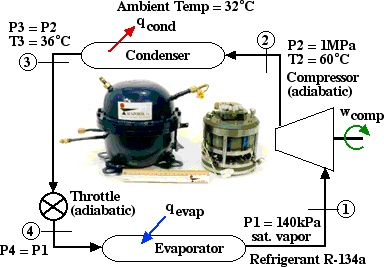
\includegraphics[width=0.75\textwidth]{ch4_hw_refrig}
  \end{center}
  \begin{questionparts}
  \item Neatly sketch the complete cycle on the pressure-enthalpy $p$-$h$ diagram for R134a, indicating clearly all 4 stations on the diagram.
  \item Determine the work done by the compressor \answer{ [54 kJ/kg]}.
  \item Determine the heat absorbed by the evaporator \answer{ [137 kJ/kg]}, and that rejected by the condenser \answer{ [191 kJ/kg]}.
  \item Determine the Coefficient of Performance of the refrigerator ($COP_R$) (defined as the heat absorbed in the evaporator divided by the work done on the compressor - always presented as a positive value even though the work done $w_c$ is negative) \answer{[$COP_R$ = 2.53]}.
  \end{questionparts}
  \newpage
  \question It is common practice in the refrigeration industry to use an internal heat exchanger to subcool the refrigerant at the outlet of the condenser by means of the refrigerant exiting the evaporator. This practice obtains a much larger refrigeration capacity using the same components.

  Continuing the previous problem, we will add a heat exchanger as indicated.
  \begin{center}
    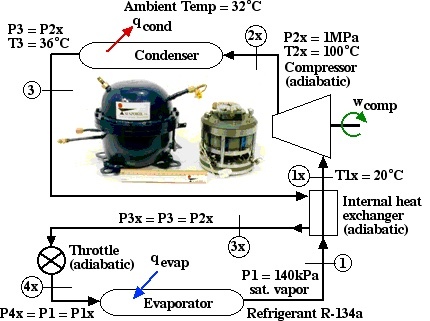
\includegraphics[width=0.75\textwidth]{ch4_HW_refrigHX}
  \end{center}

  Notice that we have included an internal heat exchanger that heats the refrigerant exiting the evaporator (as a saturated vapor at 140kPa) to 20°C. We have chosen a state numbering system (1x, 2x, and so on) so as to allow the new system to be plotted on the same $p$-$h$ diagram as above, and thus to be able to qualitatively compare the increase and improvement of performance provided by adding the internal heat exchanger.
  \begin{questionparts}
  \item Add the 4 states (1x, 2x, 3x, 4x) to the pressure-enthalpy $p$-$h$ diagram from the previous problem and sketch the new cycle.
  \item Determine the heat transferred in the internal heat exchanger, assuming it to be externally adiabatic \answer{ [32.2 kJ/kg]}, and the temperature of the subcooled liquid entering the throttle (3x) \answer{[13.4°C]}.  The heat transferred can be calculated through the equation:
    \begin{equation*}
      q = h_{1x} - h_1 = h_3 - h_{3x}
    \end{equation*}
  \item Determine the heat absorbed by the evaporator \answer{[169 kJ/kg]}.
  \item Determine the heat rejected by the condenser \answer{[235 kJ/kg]}.
  \item Determine the Coefficient of Performance of the refrigerator ($COP_R$) (defined as the heat absorbed in the evaporator divided by the work done on the compressor) \answer{[$COP_R$ = 2.65].}
  \end{questionparts}

  \newpage
  \question We wish to do a preliminary thermodynamic evaluation of a 1kW input power home heat pump system for space heating using refrigerant R134a. Consider the following system flow diagram:
  \begin{center}
    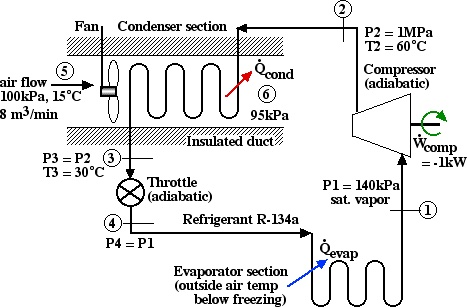
\includegraphics[width=0.75\textwidth]{ch4_HW_heatpump}
  \end{center}

  Thus the heat pump system absorbs heat from the evaporator placed outside in order to pump heat into the air flowing through the insulated duct over the condenser section. The fan provides an air flow of 8 ${\rm m^3/min}$, which is enough to cool the refrigerant in the condenser to 30°C, In this analysis we will neglect the power provided to the fan. We also assume that the duct is adiabatic, and that all the heat rejected by the condenser is absorbed by the air flowing in the duct.

  \begin{questionparts}
  \item Neatly sketch the complete cycle on the pressure-enthalpy $p$-$h$ diagram for R134a, indicating clearly all 4 stations on the diagram (stations 5 and 6 are air, and are therefore not on the same $p$-$h$ diagram).
  \item Determine the mass flow rate of the refrigerant R134a \answer{[0.0185kg/s]}.
  \item Determine the mass flow rate of the air flowing in the insulated duct \answer{[0.161kg/s]}.
  \item Determine the heat rejected by the condenser \answer{[3.7kW]}. Assuming that all this heat is absorbed by the air, determine the exit temperature of the air at station (6) \answer{[37.9°C]}. Is this value reasonable? Why?
  \item Determine the heat absorbed by the evaporator \answer{[2.7kW]}.
  \item Determine the Coefficient of Performance of the heat pump ($COP_{HP}$) (defined as the heat rejected by the condenser divided by the work done on the compressor) \answer{[3.7]}.
  \end{questionparts}

  \newpage
  \question We wish to do a preliminary thermodynamic evaluation of a 500W input power home heat pump system as applied to summertime use for both hot water heating to 50°C, and space cooling (air conditioning), and thus maintain the inside home temperature at a comfortable 20°C.

  \begin{center}
    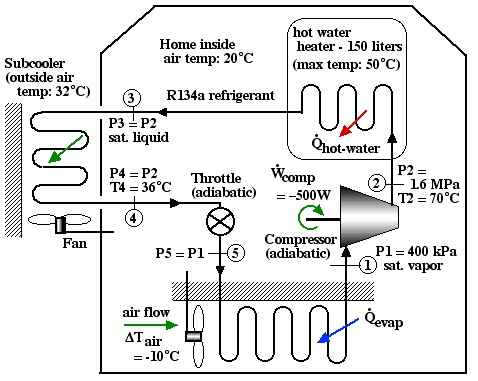
\includegraphics[width=0.75\textwidth]{ch4_HW_AC}
  \end{center}

  This unique combined air conditioning / hot water heating system is designed to absorb heat from the air flowing through the insulated duct in order to pump heat into the hot water heating tank. The fan provides enough air flow over the evaporator to cool the air by 10°C as it passes through the duct, and the hot water is heated to a maximum of 50°C. In this analysis we neglect the power provided to the fan. We also assume that both the duct and the hot water tank are externally adiabatic.
  
  \begin{questionparts}
  \item Neatly sketch the complete cycle on the pressure-enthalpy $p$-$h$ diagram for R134a, indicating clearly all 5 stations on the diagram.
  \item Determine the enthalpy values at all five stations [kJ/kg], and indicate these values on the $p$-$h$ diagram.
  \item Determine the mass flow rate of the refrigerant R134a \answer{[0.0133 kg/s]}.
  \item Determine the heat rejected by the condenser \answer{[2.09 kW]}. Assuming that all this heat is absorbed by the water in the hot water tank, determine the time taken for 150 liters of water at 30°C to reach the required temperature of 50°C \answer{[1 hr 40 min]}.
  \item Determine the heat power absorbed by the refrigerant in the evaporator \answer{[2.04 kW]}. Assuming that all this heat is absorbed from the air in the duct and neglecting the fan power, determine the required mass flow rate of the in order reduce the air temperature by 10°C while passing through the duct \answer{[0.204 kg/s]}.
  \item Determine the Coefficient of Performance of the hot water heater ($COP_{HW}$) (defined as the heat rejected by the condenser divided by the work done on the compressor) \answer{[$COP_{HW}$ = 4.17]}.
  \item Determine the Coefficient of Performance of the air conditioner ($COP_{AC}$) (defined as the heat absorbed by the evaporator divided by the work done on the compressor) \answer{[$COP_{AC}$ = 4.07]}.
  \item If we bypass the outside subcooler (State (4) becomes saturated liquid as in State (3)) determine the change in Coefficient of Performance of the air conditioner evaluated above. Indicate this change on the $p$-$h$ diagram and discuss the relevance of the outside subcooling section in this system. \answer{[$COP_{AC}$ reduced to 3.17]}.
  \end{questionparts}
\end{homework}
